\documentclass[12pt]{article}
\usepackage{latexsym,amssymb,amsmath} % for \Box, \mathbb, split, etc.
% \usepackage[]{showkeys} % shows label names
\usepackage{cite} % sorts citation numbers appropriately
\usepackage{path}
\usepackage{url}
\usepackage{verbatim}
\usepackage[pdftex]{graphicx}

% horizontal margins: 1.0 + 6.5 + 1.0 = 8.5
\setlength{\oddsidemargin}{0.0in}
\setlength{\textwidth}{6.5in}
% vertical margins: 1.0 + 9.0 + 1.0 = 11.0
\setlength{\topmargin}{0.0in}
\setlength{\headheight}{12pt}
\setlength{\headsep}{13pt}
\setlength{\textheight}{625pt}
\setlength{\footskip}{24pt}

\renewcommand{\textfraction}{0.10}
\renewcommand{\topfraction}{0.85}
\renewcommand{\bottomfraction}{0.85}
\renewcommand{\floatpagefraction}{0.90}

\usepackage{accents}
\newcommand{\ubar}[1]{\underaccent{\bar}{#1}}
\makeatletter
\setlength{\arraycolsep}{2\p@} % make spaces around "=" in eqnarray smaller
\makeatother
\usepackage{stackengine}
% change equation, table, figure numbers to be counted inside a section:
\numberwithin{equation}{section}
\numberwithin{table}{section}
\numberwithin{figure}{section}

% begin of personal macros
\newcommand{\half}{{\textstyle \frac{1}{2}}}
\newcommand{\eps}{\varepsilon}
\newcommand{\myth}{\vartheta}
\newcommand{\myphi}{\varphi}

\newcommand{\IN}{\mathbb{N}}
\newcommand{\IZ}{\mathbb{Z}}
\newcommand{\IQ}{\mathbb{Q}}
\newcommand{\IR}{\mathbb{R}}
\newcommand{\IC}{\mathbb{C}}
\newcommand{\Real}[1]{\mathrm{Re}\left({#1}\right)}
\newcommand{\Imag}[1]{\mathrm{Im}\left({#1}\right)}
\DeclareRobustCommand{\brkbinom}{\genfrac[]{0pt}{}}
\newcommand{\norm}[2]{\|{#1}\|_{{}_{#2}}}
\newcommand{\abs}[1]{\left|{#1}\right|}
\newcommand{\ip}[2]{\left\langle {#1}, {#2} \right\rangle}
\newcommand{\der}[2]{\frac{\partial {#1}}{\partial {#2}}}
\newcommand{\dder}[2]{\frac{\partial^2 {#1}}{\partial {#2}^2}}
\usepackage{enumitem}
\newcommand{\nn}{\mathbf{n}}
\newcommand{\xx}{\mathbf{x}}
\newcommand{\uu}{\mathbf{u}}
\usepackage{tikz}
\usetikzlibrary{arrows}
\usetikzlibrary{positioning}
\usepackage{titlesec}
\newcommand{\junk}[1]{{}}
\usepackage{sectsty}
\usepackage{xcolor}
\newcommand*{\bfrac}[2]{\genfrac{}{}{0pt}{}{#1}{#2}}
\newcommand\myatop[2]{\left[{{#1}\atop#2}\right]} % "wrapper macro"
\usepackage{array}
\usepackage{multirow}
\usepackage{amsmath}
\DeclareMathOperator*{\argmax}{arg\,max}
\DeclareMathOperator*{\argmin}{arg\,min}
\makeatletter
\renewcommand*\env@matrix[1][\arraystretch]{%
	\edef\arraystretch{#1}%
	\hskip -\arraycolsep
	\let\@ifnextchar\new@ifnextchar
	\array{*\c@MaxMatrixCols c}}
\makeatother

\makeatletter
\renewcommand*\env@matrix[1][*\c@MaxMatrixCols c]{%
	\hskip -\arraycolsep
	\let\@ifnextchar\new@ifnextchar
	\array{#1}}
\makeatother

\definecolor{darkblue}{rgb}{0,0,0.4}
\usepackage[colorlinks = true,
linkcolor = darkblue,
urlcolor  = darkblue,
citecolor = darkblue,
anchorcolor = darkblue]{hyperref}
% set two lengths for the includegraphics commands used to import the plots:
\newlength{\fwtwo} \setlength{\fwtwo}{0.45\textwidth}
% end of personal macros

\begin{document}
\DeclareGraphicsExtensions{.jpg}

\begin{center}
\textsc{\Large Statistical Pattern Recognition} \\[2pt]
	\textsc{\large Assignment 6}\\
	\vspace{0.5cm}
  Ali Gholami \\[6pt]
  Department of Computer Engineering \& Information Technology\\
  Amirkabir University of Technology  \\[6pt]
  \def\UrlFont{\em}
  \url{https://aligholamee.github.io}\\
    \href{mailto:aligholami7596@gmail.com}{\textit{aligholami7596@gmail.com}}
\end{center}

\begin{abstract}

\end{abstract}

\subparagraph{Keywords.} \textit{}


\section{LDF Based on Perceptron Learning Rule}
Recall that a perceptron learns a linear classifier with weight vector $W$. It predicts:
$$
	\hat{y} = sign(W^Tx_t) 
$$
assuming here that $ \hat{y} \in \{+1, -1\} $. When the perceptron makes a mistake, it updates the weights using the formula:
$$
	W^{t + 1} = W^t + y_tx_t
$$
Imagine that we have $x_t \in I^2$, and we encounter the following data points:
$$
\begin{tabular}{ | l | c | r |}
\hline	
X[1] & X[2] & y \\ \hline		
1 & 1 & 1 \\
2 & -1 & -1 \\
-3 & -1 & -1 \\
-3 & 1 & 1 \\
\hline  
\end{tabular}
$$
\begin{enumerate}[label=(\alph*)]
	\item Starting with $W = [0\ 0]^T$, use the Perceptron Algorithm to learn on the data points in the order from top to bottom. Show the Perceptron's linear decision boundary after observing each data point. Be sure to show which side is classified as positive.
	
	\item Does our learned perceptron maximize the margin between the training data and the decision boundary? If not, draw the maximum-margin decision boundary.
\end{enumerate}
\subsection*{Solution}
We'll start by augmenting the feature vectors given in the table. We'll add a new feature $x_0$ (bias term) and set it to $1$ for class $1$, and $-1$ for class $-1$. This results in the following data points:
$$
\begin{tabular}{ | l | l | c | r |}
	\hline	
	Y[0] & Y[1] & Y[2] & Class \\ \hline		
	1 & 1 & 1 & 1 \\
	-1 & -2 & 1 & -1 \\
	-1 & 3 & 1 & -1 \\
	1 & -3 & 1 & 1 \\
	\hline  
\end{tabular}
$$
we'll then augment the weight vector for a consistent definition of the decision boundary. The yields in
$$
 	W = \begin{bmatrix}
	0 \\
	0 \\
	\end{bmatrix}\ \rightarrow\  	a^0 = \begin{bmatrix}
	0 \\
	0 \\
	0 \\
	\end{bmatrix} 
$$
Note that according to the Perceptron Learning Rule, we're looking for a line to meet the following constraint:
\begin{equation}
	z_i = a^Ty_i > 0\ \  \forall y_i
\end{equation}
weights $a = \begin{bmatrix}
0 \\
0 \\
0 \\
\end{bmatrix} $ cannot correctly classify the first point since $z_1^0 = 0$ which is a sign of misclassification. We can correctly classify this point conducting a \textit{weight update} using Perceptron Learning Rule:
$$
	a^1 = \begin{bmatrix}
	0 \\
	0 \\
	0 \\
	\end{bmatrix} + \begin{bmatrix}
	1 \\
	1 \\
	1 \\
	\end{bmatrix} = \begin{bmatrix}
	1 \\
	1 \\
	1 \\
	\end{bmatrix}
$$
The resulting linear boundary will incorrectly classify the second point:
$$
	z_2^2 = \begin{bmatrix}
	1 & 1 & 1\\
	\end{bmatrix}.\begin{bmatrix}
	-1 \\
	-2 \\
	1 \\
	\end{bmatrix} \leq 0
$$
Thus we have to update the weights using Perceptron Rule again:
$$
	a^2 = \begin{bmatrix}
	1 \\
	1 \\
	1 \\
	\end{bmatrix} + \begin{bmatrix}
	-1 \\
	-2 \\
	1 \\
	\end{bmatrix} = \begin{bmatrix}
	0 \\
	-1 \\
	2 \\
	\end{bmatrix}
$$
The resulting line will poorly perform on the third data point:
$$
z_3^3 = \begin{bmatrix}
-1 & 3 & 1\\
\end{bmatrix}.\begin{bmatrix}
0 \\
-1 \\
2 \\
\end{bmatrix} \leq 0
$$
Updated weights for the third iteration is provided below:
$$
	a^3 = \begin{bmatrix}
	0 \\
	-1 \\
	2 \\
	\end{bmatrix} + \begin{bmatrix}
	-1 \\
	3 \\
	1 \\
	\end{bmatrix} = \begin{bmatrix}
	-1 \\
	2 \\
	3 \\
	\end{bmatrix}
$$
following the same pattern for the final data point results in the final weight update:
$$
	a^4 = \begin{bmatrix}
	0 \\
	-1 \\
	2 \\
	\end{bmatrix} + \begin{bmatrix}
	1 \\
	-3 \\
	1 \\
	\end{bmatrix} = \begin{bmatrix}
	1 \\
	-4 \\
	3 \\
	\end{bmatrix}
$$
Corresponding decision boundaries for each step is provided in the figure 1.1

\begin{figure}[!h]\centering
	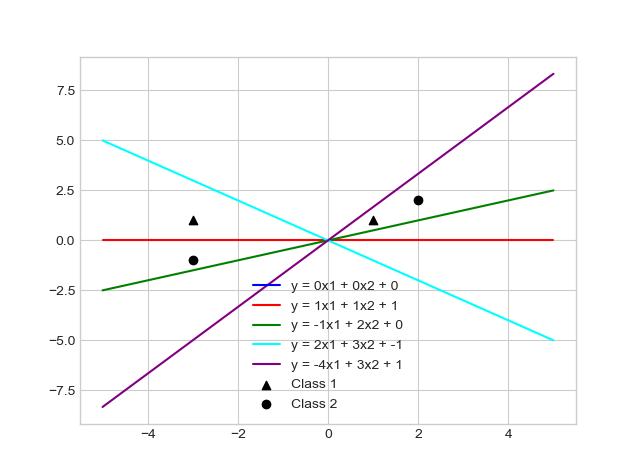
\includegraphics[width=0.7\textwidth]{plot_1.PNG}
	\caption{Illustration of Perceptron decision boundaries and class points.}
	\label{pl1}
\end{figure}

The learned Perceptron does not maximize the margin between the training data and the decision boundary. The max-margin linear discriminator is $y = 0$.
\section{Perceptron in Practice}
Start with the truth tables for boolean \textit{AND} and \textit{OR}. Your goal is to write an small program to train a \textit{two-input one-output} Perceptron using this data. Select some random initial weights in the interval $(0, 1)$. Use a learning parameter $0.1$. The stopping condition is 50 iterations or \textit{no change in weights from one epoch to the next}, whichever comes first.
\begin{enumerate}[label=(\alph*)]
	\item Encode \textit{FALSE = 0} and \textit{TRUE = 1} for the input values. Remember that the output of a Perceptron, by definition is $+1$ or $-1$.
	\item Encode \textit{FALSE = -1} and \textit{TRUE = +1} for the input values. Remember that the output of a Perceptron, by definition is $+1$ or $-1$.
\end{enumerate}
For each case, please show the evolution in the change of weights by arranging them in a nice tabular format. Remember to include the weight $w_0$ as a part of the training process and set your $x_0$ to $+1$ all the time. For each case, please plot the separating hyperplane in the $x_1-x_2$ plane. Submit your code, result of your run and your comments.

\section{Support Vector Machine}
Consider a dataset with 2 points in $1D$:
$$
	X_1 = 0,\ Y_1 = -1 \ \ \ \ X_2 = \sqrt{2},\ Y_2 = 1
$$
Consider mapping each point to $3D$ using the feature vector $\phi(x) = [1,\ \sqrt{2}x,\  x^2]^T$. Here, the max margin classifier has the form:
\begin{equation}
	\hat{W},\ \hat{W_0} = argmin||W||^2
\end{equation}
so that
$$
	y_1(W^T\phi_1(x) + W_0) \geq 1
$$
$$
	y_2(W^T\phi_2(x) + W_0) \geq 1
$$
\begin{enumerate}[label=(\alph*)]
	\item Write down a vector that is parallel to the optimal vector $\hat{W}$. Hint: $\hat{W}$ is prependicular to the decision boundary between the two points in the $3D$ feature space.
	
	\item What is the value of the margin that is achieved by this $\hat{W}$? Hint: The margin is the distance from each support vector to the decision boundary. Think about the geometry of the points in feature space, and the vector between them.
	
	\item Solve for $\hat{W}$, using the fact that the margin is equal to $\frac{1}{||\hat{W}||}$.
	
	\item Solve for $\hat{W_0}$ using your value for $\hat{W}$ and (3.1). Hint: The points will be on the decision boundary, so the inequalities will be tight. A \textit{Tight Inequality} is an equality that is as strict as possible.
\end{enumerate}

\subsection*{Solution}
The initial 1-dimensional dataset is $D = (0 \ \ \sqrt{2})$. Applying the transformation yields the following points in $3D$:
$$
	D' = \begin{bmatrix}
	1 & 1 \\
	0 & 2 \\
	0 & 2 \\
	\end{bmatrix}
$$
In order to find the \textit{SVM} decision boundary, we'll use the following formula which represents an optimization problem with respect to the constraints given in the problem description:
\begin{equation}
	L_D(\alpha) = \sum_{i = 1}^{2}\alpha_i - \frac{1}{2}\sum_{i = 1}^{2}\sum_{i = 1}^{2}\alpha_i\alpha_jz_iz_jx_i.x_j
\end{equation}
This can be written as
$$
	L_D(\alpha) = \alpha_1 + \alpha_2 - \frac{1}{2}(\alpha_1\begin{bmatrix}
	1 \\ 
	0 \\
	0 \\
	\end{bmatrix} - \alpha_2\begin{bmatrix}
	1 \\ 
	2 \\
	2 \\
	\end{bmatrix}).(\alpha_1\begin{bmatrix}
	1 \\ 
	0 \\
	0 \\
	\end{bmatrix} - \alpha_2\begin{bmatrix}
	1 \\ 
	2 \\
	2 \\
	\end{bmatrix})
$$
simplifying the results yields in 
\begin{equation}
		L_D(\alpha) = \frac{-9}{2}\alpha_2^2 - \frac{1}{2}\alpha_1^2 + \alpha_1\alpha_2 + \alpha_1 + \alpha_2
\end{equation}
To solve (3.3), we should find the derivatives with respect to $\alpha_1$ and $\alpha_2$.
$$
	\der{L_D(\alpha)}{\alpha_1} = -\alpha_1 + \alpha_2 + 1 = 0
$$
$$
	\der{L_D(\alpha)}{\alpha_2} = -9\alpha_2 + \alpha_1 + 1 = 0
$$
Thus $\alpha_1 = \frac{5}{4}$ and $\alpha_2 = \frac{1}{4}$. Weights can be obtained using
\begin{equation}
	W = \sum_{i = 1}^{2}z_ix_i\alpha_i
\end{equation}
Thus
$$
	W = \frac{5}{4}\begin{bmatrix}
	1 \\
	0 \\
	0 \\
	\end{bmatrix} - \frac{1}{4}\begin{bmatrix}
	1 \\
	2 \\
	2 \\
	\end{bmatrix} = \begin{bmatrix}
	1 \\
	-1/2 \\
	-1/2 \\
	\end{bmatrix}
$$
An obvious vector parallel with the weight vector is the normalized vector of W:
$$
	V = \begin{bmatrix}
	\frac{1}{\sqrt{1 + \frac{1}{4} + \frac{1}{4}}} \\
	\frac{\frac{-1}{2}}{\sqrt{1 + \frac{1}{4} + \frac{1}{4}}} \\
	\frac{\frac{-1}{2}}{\sqrt{1 + \frac{1}{4} + \frac{1}{4}}} \\	
	\end{bmatrix} = \begin{bmatrix}
	 0.81 \\
	-0.40 \\
	-0.40 \\	
	\end{bmatrix}
$$
\section{Hierarchical Clustring}
Let $X = \{x_i,\ i = 1, 2, 3, 4, 5 \}$, with $x_1 = [1,\ 1]^T$, $x_2 = [2,\ 1]^T$, $x_3 = [5,\ 4]^T$, $x_4 = [6,\ 5]^T$ and $x_5 = [6.5,\ 6]^T$. The pattern matrix of X is
$$
	D(X) = \begin{bmatrix}
	1 & 1\\
	2 & 1\\
	5 & 4\\
	6 & 5\\
	6.5 & 6\\
	\end{bmatrix}
$$
Use the following methods to cluster the pattern matrix and draw the dendogram for hierarchical models:
\begin{enumerate}[label=(\alph*)]
	\item Single Linkage
	\item Complete Linkage
	\item Average Linkage
	\item Mean Method
\end{enumerate}
\end{document} 



